\chapter{Mises à jour de l'expérience}
\label{ch:new_exp}
%\begin{tikzpicture}[remember picture, overlay]
%\node[anchor=north east,inner sep=0pt] at (current page.north east) {
\includegraphics[scale=1]{Fig/Chapter1/g825.png}};
%\end{tikzpicture}

Nous avons vu dans le chapitre précédent comment, expérimentalement, nous pouvons créer une onde de matière obtenue par la condensation de Bose-Einstein. Nous avons ainsi présenté les principaux outils dont nous disposons pour manipuler les atomes et la manière dont nous en tirons profit sur notre dispositif. Une telle plateforme recquiert une quantité importante de matériels variés qu'il est nécessaire d'entretenir, de réparer, voire de remplacer. 

Dans ce nouveau chapitre, nous nous pencherons sur les modifications apportées à l'expérience au cours de ma thèse. Dans la première partie, nous parlerons d'informatique et plus particulièrement du contrôle de l'expérience. Dans un second temps, nous caractériserons la lévitation magnétique suite à une avarie sur le circuit de refroidissement à eau. Ensuite, nous calibrerons le piège dipolaire dont le laser source a été changé. Pour terminer, nous discuterons de l'amélioration de l'évaporation optique permise par les changements précédents.

\section{Mise à jour de l'informatique de l'expérience}
Souvent absente des présentations des expériences, l'informatique occupe pourtant une place primordiale dans les dispositifs d'atomes ultra-froids. Le contrôle simultané et de manière séquentielle des différents équipements de l'expérience, souvent précis à la micro-seconde, n'est possible qu'à l'aide d'un ordinateur disposant de sorties de tension controllables. Cet ordinateur, appelé \emph{séquenceur}, constitue le cerveau de l'ensemble du dispositif et contrôle tous les éléments nécessaires à la manipulation des atomes.

Le second aspect où l'informatique se rend indispensable réside dans l'acquisition et le traitement d'images. Le contrôle des caméras et l'extraction des quantités physiques à partir d'images expérimentales nécessite l'utilisation d'un ordinateur et d'au moins un logiciel adapté. 

De manière générale, les ordinateurs sont les éléments du dispositif avec lesquels l'expérimentateur intéragit le plus. Dans cette partie, on présentera donc les changements informatiques ayant eu lieu durant ma thèse.

\subsection{Contrôle de l'expérience: passage à la suite Cicero}
\label{sc:cicero}
Une modification majeure a été le changement du séquenceur de l'expérience. Le précédent système développé par André Villing, ingénieur électronicien du laboratoire maintenant retraité, était piloté de manière programmatique depuis le logiciel Matlab. À des fins de maintenance, le nouveau séquenceur est d'origine commerciale et est basé sur du matériel \emph{National Instruments}:
\begin{itemize}
\item[\textendash] Un ordinateur \emph{PXIe-8840} dans un chassis \emph{PXIe-1078} qui alimente aussi les cartes de génération de signaux.
\item[\textendash] Deux cartes numériques \emph{PXIe-6535} de 32 voies chacune.
\item[\textendash] Deux cartes analogiques \emph{PXIE-6738} de 32 voies $\pm10$V chacune et codées sur 16 bits.
\end{itemize}
En addition, un circuit logique programmable (\emph{FPGA}) \emph{XEM3001} provenant de \emph{Opal-Kelly} permet de générer une horloge de fréquence variable pour le matériel \emph{National Instruments}. La justification de cette horloge de fréquence variable réside dans la grande variabilité de la durée des différentes étapes d'une expérience d'atomes ultra-froids: l'expérience peut rester dans le même état plusieurs secondes (pendant le chargement d'un MOT par exemple) tout comme elle doit pouvoir changer d'état pendant quelques microsecondes seulement (pendant l'imagerie par exemple). Une séquence durant typiquement 30s discrétisée toutes les microsecondes saturerait alors la mémoire de l'ordinateur. 

L'écriture de la séquence se fait à présent grâce à la suite \emph{Cicero Word Generator}, développée au \emph{MIT} dans le groupe de Wolfgang Ketterle \citep{keshet2013distributed}. Cette suite comporte deux logiciels qui fonctionnent selon une architecture client/serveur. Le client \emph{Cicero} est une interface graphique dans laquelle l'utilisateur écrit une séquence sous la forme d'une suite d'étapes comme illustré figure \ref{fig:cicero}. Au lancement d'un cycle expérimental, \emph{Cicero} envoie les données de séquence au serveur \emph{Atticus} qui calcule alors les consignes des cartes ainsi que l'horloge variable à appliquer \citep{keshet2008cicero}.

\begin{figure}
\centering
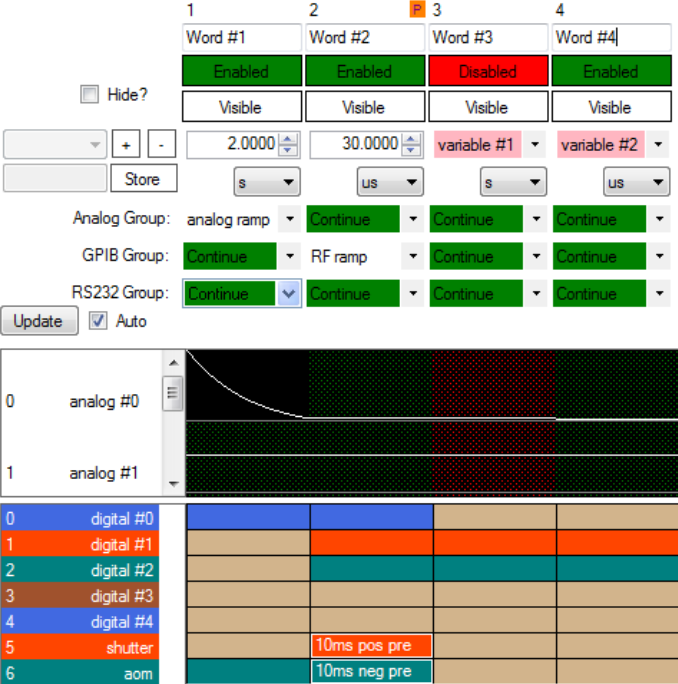
\includegraphics[width=0.7\textwidth]{Fig/Modif_exp/cicero.png}
\caption{\textbf{Capture d'écran de \emph{Cicero}.} Une séquence est une suite d'étapes (des colonnes dans l'interface) pendant lesquelles on peut faire des motifs avec les voies analogiques. Les voies numériques changent d'état en général entre deux étapes. Il est possible de désactiver certaines étapes et d'utiliser des variables. Figure tirée de \citep{keshet2013distributed}.}
\label{fig:cicero}
\end{figure}

Grâce à cette architecture client/serveur, il est possible de connecter une interface \emph{Cicero} à plusieurs serveurs. Nous avons ainsi développé un serveur supplémentaire\footnote{Une attention particulière a été accordée à n'apporter aucune modification au code source de la suite \emph{Cicero} excepté dans l'environnement de ce serveur. Les environnements de \emph{Cicero}, \emph{Atticus} et les environnements communs n'ont subit aucun changement pour s'assurer de la compatibilité avec la version compilée 1.64rev7 de la suite.} afin de faciliter notre traitement de données. Celui-ci enregistre les principales données de séquence\footnote{Il s'agit du nom de séquence, de l'heure de lancement, de l'ensemble des variables, des étapes, des groupes d'étapes et de la dernière consigne du piège dipolaire avant le temps de vol.} à chaque cycle.

Ce changement de séquenceur ouvre de nouvelles perspectives en augmentant le nombre de voies utilisables (16 voies analogiques codées sur 12 bits et 48 voies numériques avec le précédent système) tout en permettant la génération de signaux arbitraires (auparavant limités à des morceaux de rampes).


\subsection{Développement d'une nouvelle interface d'acquisition et de traitement d'images}
Comme présenté dans la partie \ref{sc:imagerie}, les caméras que l'on utilise sur l'expérience sont configurées et contrôlées via le logiciel Matlab. En particulier, l'acquisition et le traitement des images se faisait à l'aide d'une interface commune avec l'ancien séquenceur. Son remplacement a donc eu un impact important sur le fonctionnement de la partie imagerie. 

En conséquence, nous avons réalisé une nouvelle interface graphique permettant de configurer les caméras, d'acquérir et de traiter les images, d'enregistrer les données et de contrôler tout les éléments non adressables depuis \emph{Cicero}. Le cahier des charges de cette nouvelle interface est donc le suivant:
\begin{itemize}
\item[\textendash] Gestion des trois caméras, avec possibilité de faire l'acquisition simultanée sur les deux caméras de la chambre de science\footnote{Un ordinateur supplémentaire était nécessaire pour le contrôle de la caméra \textit{bottom}, pilotée via une autre interface. Il fallait donc synchroniser ces deux ordinateurs qui enregistraient chacun leurs fichiers de données.}.
\item[\textendash] Imagerie par absorption et par fluorescence.
\item[\textendash] Calcul des grandeurs physiques pour chaque image.
\item[\textendash] Lecture des données de Cicero récupérées grâce au serveur que nous avons développé.
\item[\textendash] Programmation en début de cycle des sources radio-fréquence utilisées pour l'évaporation radio-fréquence et la manipulation de l'état de spin dans la chambre de science\footnote{Cette programmation en début de cycle est rendue possible grâce à l'utilisation d'un \emph{FileSystemWatcher} provenant d'une bibliothèque .NET utilisable dans Matlab. Un fichier texte contenant les données du cycle en cours est généré en début de séquence par le serveur que nous avons développé, déclenchant alors automatiquement sa lecture par l'interface.}.
\item[\textendash] Enregistrement de l'ensemble des données et des paramètres du cycle pour un futur traitement.
\end{itemize}
L'utilisation de cette nouvelle interface a donc permit de centraliser les données générées par l'acquisition d'images en n'ayant plus besoin d'un ordinateur supplémentaire (et de la synchronisation associée). 











\section{Réparation et recalibration de la lévitation magnétique}
\label{sc:levitation}
Comme présenté partie \ref{sc:chambre_science}, la lévitation magnétique est un élément essentiel de notre expérience. En plus d'être un pré-requis pour l'étude de la localisation d'Anderson à trois dimensions, celle-ci nous permet de manière générale d'obtenir des échantillons particulièrement froids. Son bon fonctionnement est donc une priorité pour notre expérience.

MOUUUUUAAAAAAIIIIIIIS. Dans cette partie, nous présenterons dans un premier temps notre système de lévitation. Enfin, nous nous pencherons sur les méthodes utilisées pour calibrer le système après sa réinstallation sur l'expérience. MOOOOOUUUUAAAAAAAIIIIISS....

\begin{equation}
\mathbf{B}=\left( \frac{b'}{2}x \right) \vec{x} + \left[ B_0 - b'y + b'' \left( y^2 - \frac{x^2+z^2}{2} \right) \right] \vec{y} + \left( \frac{b'}{2}z \right) \vec{z}
\end{equation}



\subsection{Réparation de la lévitation magnétique}
Avarie avec le système de refroidissement à eau. Test d'étanchéité "à sec", on a trouvé des fuites qui proviendraient de l'intérieur, non trouvées même à l'aide d'un endoscope. Tentative d'étanchéité à l'aide d'une résine, non concluante. Perçage pour faire déboucher deux parties du conduit, et installation de deux barreaux de cuivre. Solution retenue. Graphe élévation de température.
Courbes résistance et temps de montée/descente montrant la non-dégradation des bobines.


\subsection{Calibration par oscillations}
\subsection{Calibration par radio-fréquences}

Déplacement du centre de la lévitation à l'aide champs de compensation.

Cette étude a permis non seulement de calibrer nos bobines dont la position, l'orientation et le comportement magnétique ont été légèrement modifiés. Mais en plus, ça nous a permit de découvrir de nouvelles limitations. 
Future nécessité de pouvoir changer les courants de compensation de manière totalement arbitraire et contrôlée en cours de séquence non réalisable avec nos alimentations actuelles: étude en cours. 















\section{Changement du laser telecom et calibration du piège optique}
Listés dans la partie \ref{sc:chambre_science}, uniquement deux éléments participent à la manipulation d'atomes dans la chambre de science avant condensation. Le premier élément, la lévitation magnétique, a fait l'objet d'un entretien essentiel présenté dans la partie précédente. 

Cette partie se concentrera sur le second élément, le piège optique. Nous commencerons par présenter le système optique et décrire les changements opérés, puis nous décrirons la calibration de ce piège sur les atomes.

\subsection{Changement du laser telecom}
Dans le chapitre précédent, nous avons vu que le piège optique était composé de deux faisceaux se croisant dans la chambre de science. 

Source commune provenant d'un laser Ytterbium 20W continu de Keopsys. Laser ancien qui a vécu, et dont la puissance n'était plus que 14W à l'allumage, pour 12.5W en fin de journée. Laser fibré, dont la taille du faisceau de sortie était de 1.4mm

Remplacement pour un nouveau laser, de chez IPG, fibré, même longueur d'onde $\lambda=1070$nm. Taille de faisceau de 0.8mm, mesuré jusqu'à 55W.

But: garder la même configuration sur les atomes: La pince ça va, c'est fibré, faut juste pas trop merder sur le mode matching à l'entrée de la fibre pour avoir la même puissance qui sort et pas cramer la fibre.
Le dimple c'est plus chiant, le chemin est direct jusqu'aux atomes via des téléscopes tubés. Beaucoup de périscopes, possibilité que l'ellipse tourne. On veut garder 180µm*90µm.


\subsection{Calibration du piège optique}
Nécessité de calibrer ce qu'il se passe au niveau des atomes. On contrôle bien ce qu'il se passe avant, mais avec le dimple on n'a pas de fibre pour fixer la taille. 

Estimation de la taille du dimple à l'aide de la divergence du faisceau derrière la cellule. Mesure à la caméra. Tailles estimée à 160*80µm. 

Mesure de la puissance. Estimation des fréquences de piégeage par ces mesures.

Mesures réelles des fréquences de piégeage dans la direction verticale $\vec{y}$ donnée par la pince et la direction horizontale $\vec{z}$ donnée par le dimple.

Mesure dans la direction verticale à l'aide de la lévitation: on dispose d'un bouton pour allumer et éteindre la gravité, et donc générer une force pendant un bref instant pour donner un mouvement aux atomes dans le piège.

Mesure dans la direction horizontale selon deux méthodes suivant la puissance. À haute puissance, on applique un gradient magnétique pour pousser les atomes à l'aides des bobines de compensations. À plus basses puissance, où le piégeage de la lévitation peut arracher les atomes de l'ODT, on éteint les bobines de compensation pour générer la force plutôt. 

Saturation pour les deux faisceaux à haute puissance, d'origines différentes. Pour la pince, il s'agit du maximum de diffraction du modulateur acousto-optique. Pour le dimple, il s'agit du maximum d'émission de la source RF. 

Variation de la puissance en allant plus ou moins loin dans l'évaporation optique.


\section{Optimisation de l'évaporation tout-optique}
\label{sc:evap_optique}

